%%% Template para anotações de aula
%%% Feito por Daniel Campos com base no template de Willian Chamma que fez com base no template de  Mikhail Klassen

\documentclass[12pt,a4paper, india]{article}

%%%%%%% INFORMAÇÕES DO CABEÇALHO
\newcommand{\workingDate}{\textsc{\selectlanguage{english}\today}}
\newcommand{\userName}{Intro. to IoT}
\newcommand{\institution}{SNU Chennai}
\usepackage{researchdiary_png}

% For Arrow Bullet Points in Lists
\usepackage{enumitem}
\newlist{arrowlist}{itemize}{1}
\setlist[arrowlist]{label=$\Rightarrow$}

% For hyperlinks
\usepackage{hyperref}

\begin{document}

\begin{center}
{\textbf {\LARGE A 2-Layered Advancement in the \\
Architecture of IoT}}\\[5mm]
{\large Abdullah Sheriff} \\[1mm]
{\normalsize AI \& DS - Section A} \\[0.8mm]
{\normalsize Roll Number: 2110220} \\[0.8mm]
{\normalsize Register Number: 21011101005} \\[0.8mm]
{\normalsize Subject: Open Elective - IoT} \\[0.8mm]
{\normalsize Semester: 4} \\[5mm]


\today\\[5mm] %% se quiser colocar data
\end{center}


\section{Topic Summary}

	The 3-layer IoT architecture (Figure 1) consisting of the Perception Layer, the Network Layer, and the Application Layer played a significant role during the inception of IoT, yet it did not completely explain its structure and connotation. 
	As IoT draws many parallels to the Communication Network and the Internet, a detailed analysis of the both of their structures was carried out by Wu et al., which enabled the formulation of an improved 5-layer IoT architecture, published in 2010.
	This research effort is a major contribution to the modern IoT infrastructure. \\

 \begin{figure}[h]
    \centering
    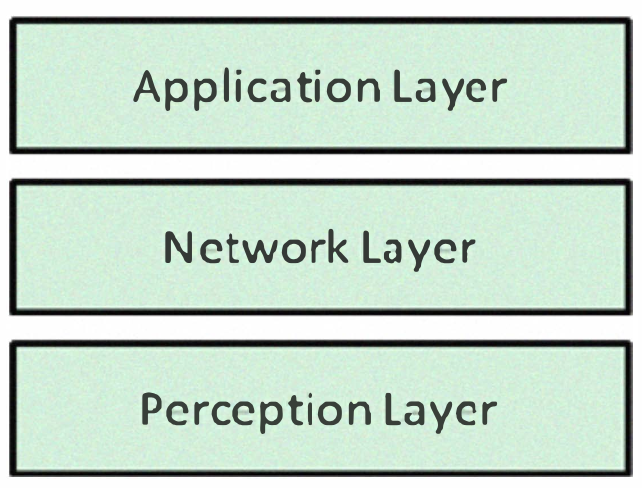
\includegraphics[width=0.25\textwidth]{3 Layer Architecture.png}
    \caption{3-layer Architecture of the Internet of Things.}
\end{figure}

\section{Key Contributions}

\begin{arrowlist}

    \item IoT’s booming development not only depends on the technology progress, but more on various new applications and successful business models.

    \item To understand the Internet of Things' system structure, it is important to analyse two network structures: the Internet and Communications Network. Although the two models are not suitable for loT directly, they have some features in common. 

    \item Through the technology architecture of the Internet and the logical structure of Telecommunications Management Network, combined with the specific features of the Internet of Things, the authors have established a new architecture of loT.

    \item IoT must be divided into 5 layers: Business, Application, Processing, Transport, and Perception Layer (Figure 2). 

    \item Perception Layer: Collect information and transform to digital signals. Many objects can not be perceived directly, so implantation of microchip into their bodies is a possibility. These chips can sense and even process information. Nanotechnology and embedded intelligence technology also are key in the Perception Layer. 

    \item Transport Layer, a.k.a., Network Layer: Transmit data using IPv6 protocol. The Internet of Things will be an immense network, which not only connects billions of things, but also encompass huge amounts of various networks. Therefore, the communication between different networks and entities is very crucial. 

    \item Processing Layer: Store, analyse, and process the information received from objects. This layer is extracted from other layers as there will exist large quantities of ‘things’, and huge volume information carried. Cloud computing and ubiquitous computing is the primary technology in this layer; For this reason, R\&D on the Processing Layer is significant for the future development of IoT.

    \item Application Layer: The task of the Application Layer is based on the data processed in the Processing Layer, and develops diverse applications of the Internet of Things, such as intelligent transportation, logistics management, identity authentication, location-based service (LBS), safety, and more.

    \item Business Layer: Manager of the Internet of Things, including managing the applications, the relevant business model and other business. It involves research on business model and profit model. This layer should manage the users' privacy, which is equally important in the IoT.

\end{arrowlist}

 \begin{figure}[h]
    \centering
    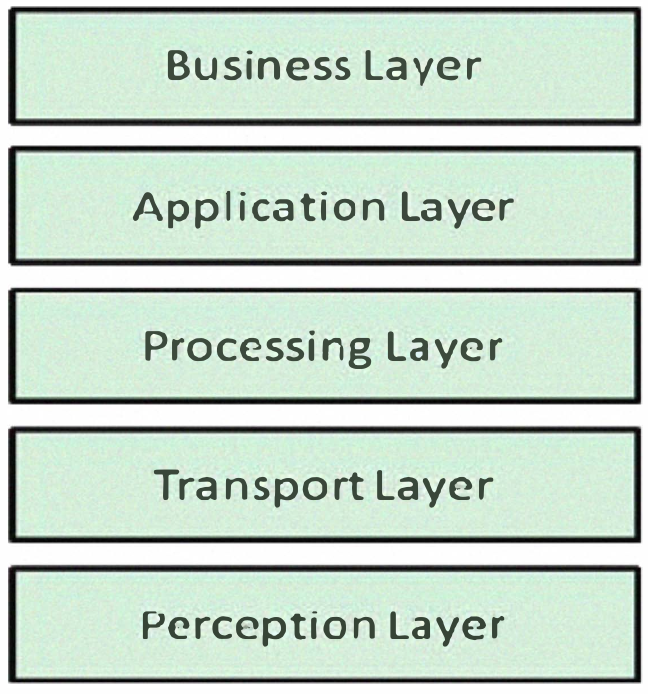
\includegraphics[width=0.25\textwidth]{5 Layer Architecture.png}
    \caption{A new 5-layer Architecture of the Internet of Things.}
\end{figure}

\section{My Views}

    Looking at IoT from a future point of view, compared to when the above paper was written, the 7-layered architecture [1] seems second-natured. The paradigm shift in the IoT architecture from 3 to 7 layers, with many in-between, has let technologies like edge computing, data mining, cryptography, and more, profoundly thrive. The situation is perfectly described by the words of late Mark Weiser, the Chief scientist at Xerox PARC,  "The most profound technologies are those that disappear. They weave themselves into the fabric of everyday life until they are indistinguishable from it". \\
    
    IoT has seeped into many products, from watches to cars. The increase in the number of layers from 3 to 5 to 7 is a product of the sheer quantity of data being collected. 
    \\

\section{Agreements, Pitfalls, and Fallacies}

    \begin{tabular}{ |p{4cm}||p{5.7cm}|p{5.7cm}|  }
    \hline
    Key Aspect / Claim & Agreement & Disagreement\\
    \hline
     
    IoT depends on Business Models.   & 
    The approach leverages creative business ideas by accelerating the expansion of IoT technology to fit the real world, rather than limiting the real-world applications by the extent of advancement in the IoT field.    &
    \\ \hline
     
    Internet and Communications Network comparison with IoT. &   
    Beautiful approach to combine 2 established domains to improve the scope of IoT.  & 
    \\ \hline

    Microchip implantation into objects. &   
    & 
    Fear that the rise of ‘embedded intelligence’ may evolve to facilitate the implantation of such microchips into humans, and enforce the same.
     
    Who or what will control the deployment of such microchips, the data collected, the functions / services provided by the chip, and more? It fatefully depends on the extent of human understanding, morals, and wisdom.
    \\ \hline

    Business layer manages User privacy. &   
    Business models control data requirements, and it seems like a good practice to enforce privacy at the ideation level.  & 
    Universal Ground rules must be laid at the Perception layer itself to prevent the of collection of sensitive data.
    \\ \hline

    IPv6 prediction. &   
    In 2011, IPV6 was publicly launched - The new protocol allowed for 2128 addresses or as Steven Leibson put it, “We could assign an IPV6 address to every atom on the surface of the earth, and still have enough addresses left to do another 100+ earths.” [2] &
    \\ \hline
    
    \end{tabular}

% Removed 'referencias.bib' and made it simple
\section{References}

\href{http://dl.icdst.org/pdfs/files4/0f1d1327c5195d1922175dd77878b9fb.pdf}{[1] http://dl.icdst.org/pdfs/files4/0f1d1327c5195d1922175dd77878b9fb.pdf}

\href{https://www.postscapes.com/iot-history/}{[2] https://www.postscapes.com/iot-history/}

\end{document}